\chapter{Expresividad}

% Aquí podría ir la parte de live coding 

\section{Live Coding} % Pregunta: Este apartatdo no debería ir antes ? En momentos anteriores menciono la cuestión  

% Antecedentes más extensos

Encuentro múltiples formas de abordar el tema. El live coding puede describirse en térrminos de unaa comunidad que realiza una práctica y que se enuncia como tal, como un sub-campo creativo que comparte elementos con otra expresiones como la música algorítmica y el arte generativo. Finalmente, el live coding podría acotarse a motivos de investigación académica e independiente y a la realización tecnlógica de interfaces de texto que corren sobre motores de audio y video.

De estas múltiples formas de abordar el fenómeno y de acuerdo a los fines de esta investigación, nos preguntamos si el eje que las articula son discusiones sobre el lenguaje y la escritura. 

\subsection{Primeras expresiones}

Antecedentes del live coding: la escena mod.

En el manifiesto del live coding se expresan pensamientos que hasta el momento, son vigentes. 

% PhD Thesis: Artist-Programmers and Programming Languages for the Arts - Alex McLean 
Dentro de los antecedentes está la experiencia performática de escribir código al vuelo con fines creativos, audiovisuales y experimentales.

Las primeras expresiones reflexivas y prácticas del live coding no solamente establecen puntos de partida performáticas, sino que al mismo tiempo aportan elementos para el diseño y análisis de sistemas basados en interfaces de código:

\begin{quote}

  ``Nuestro argumento nos lleva a través de capas de representación, comenzando con símbolos, luego palabras, lenguaje y notación, para considerar el papel que estas representaciones pueden jugar en la creatividad humana'' \citep[p.~3]{McLean2011}

\end{quote}

La noción de capas de representación permite analizar la complejidad del proceso artístico con código en términos de la relación entre humanos y los aspectos cognitivos, sociales y políticos que les atraviesan, y los no-humanos en lo que respecta a las posibilidades de conocimiento instanciado presentes en ellos. 

Live coding desde cero y la improvisación. 

\subsection{Nodos y circuitos}

La práctica de la programación al vuelo, delimitada técnica, escénica, musical y visualmente se origina en Inglaterra. % cita

Como lo describen \cite{villasenor} para los casos de Barcelona y Ciudad de México.\footnote{Un ejemplo reciente se encuentra en: \url{https://youtu.be/n5kwi4eRAE4}} 

\subsection{Exploración visual}

Exploración visual para la integración con el sonido.  

\begin{figure}[tb]
\centering 
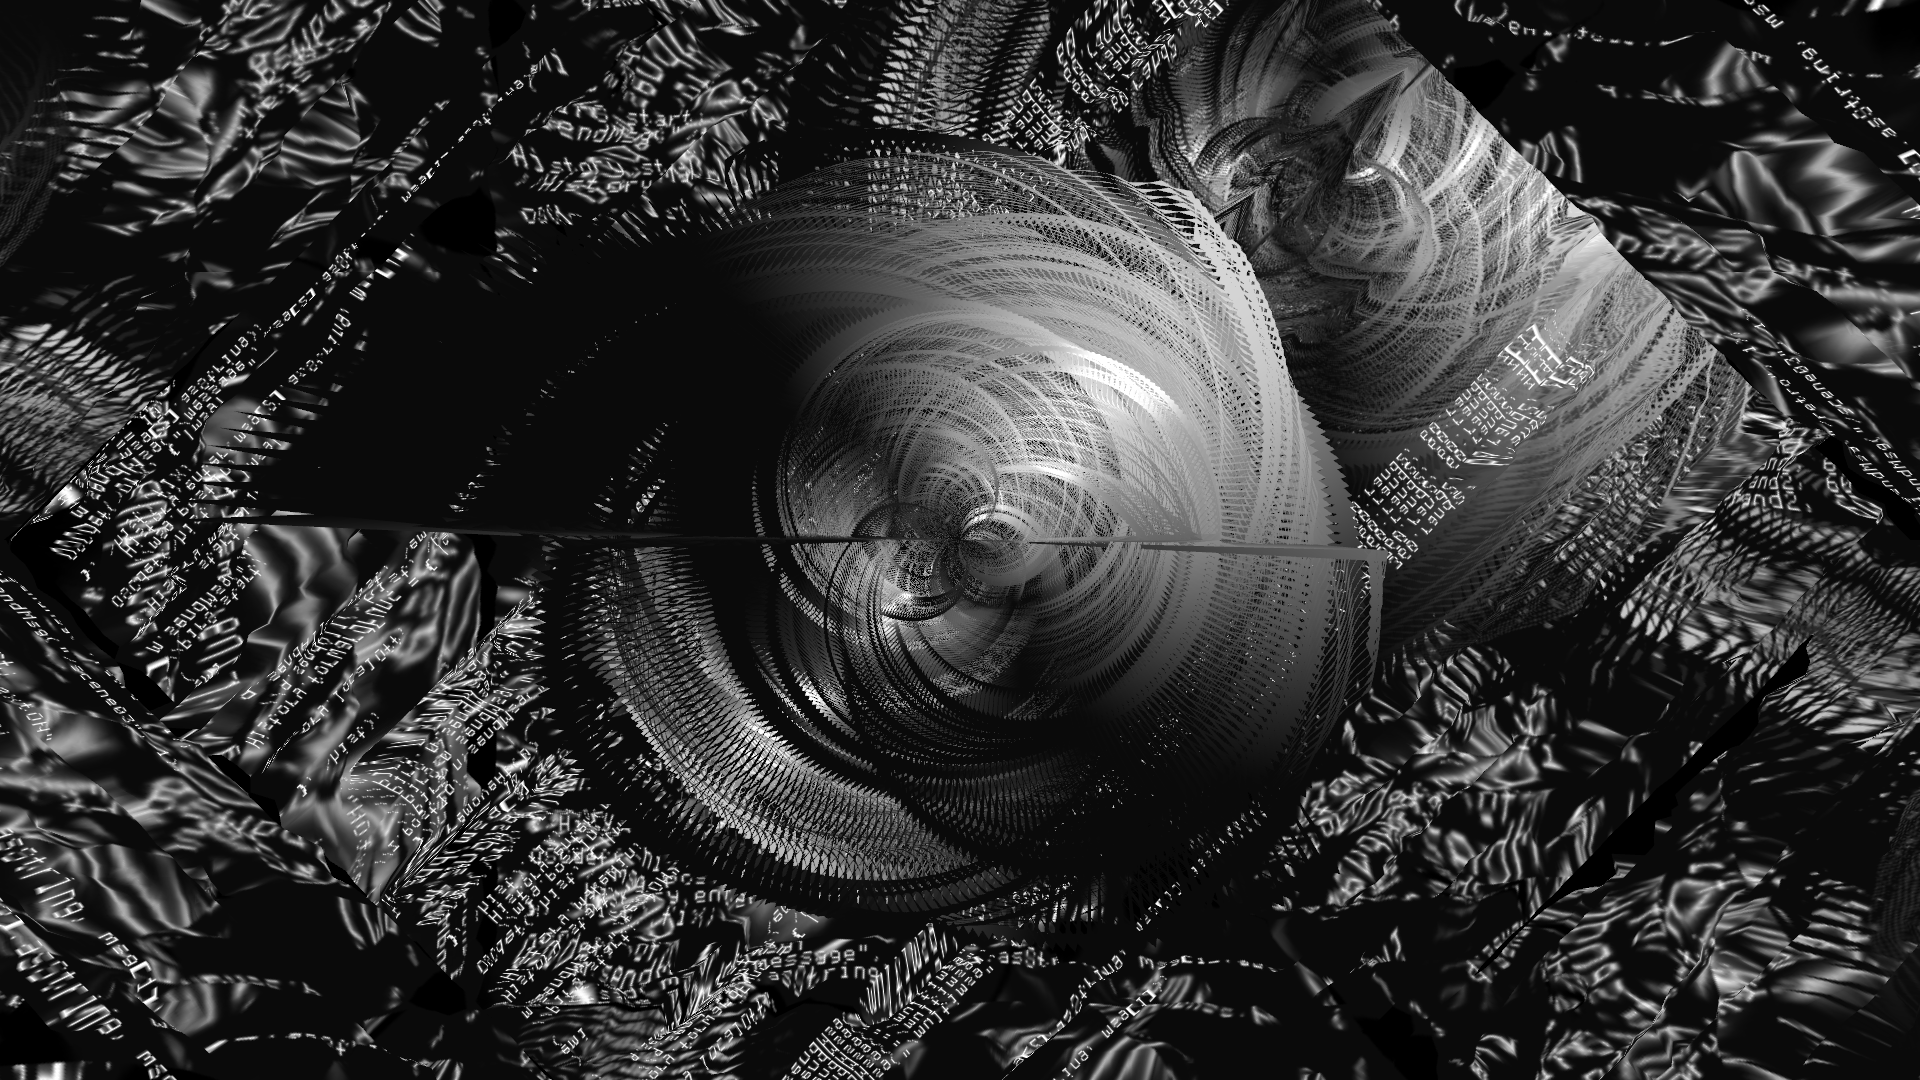
\includegraphics[width=\columnwidth]{../img/of13.png} 
\caption[Openframeworks 1]{Captura de render realizado con OpenFrameworks} % The text in the square bracket is the caption for the list of figures while the text in the curly brackets is the figure caption
\label{fig:gallery} 
\end{figure}

El campo del live coding tuvo un giro importante con la llegada de hydra de Olivia Jack. La rápida expansión de esta plataforma y la sintaxis que recuerda la conexión de flujos de energía similar a los sintetizadores analógicos favorecieron la producción de piezas e interpretaciones enfocadas en la imagen y en algunos otros casos a la par del audio. La importancia de esta plataforma ha delimitado una estética  basada en  la transformación de píxeles, de formas y de transformaciones basadas en funciones matemáticas.

En palabras de Olivia Jack, los procesos que realiza la computadora hay un eje de profundidad, en términos del despliegue gráfico físico de la computadora de espacios bi o tridimensionales, el resultado es bidimensional.

La lógica de Hydra es modular, esto quiere decir que puede incorporarse como un componente adicional a proyectos que no necesariamente se centren en la producción visual con esta plataforma. Esta modularidad juega a favor de lenguajes de programación como Javascript. 


\section{Modo estático}

Piezas fijas y la composición conducida por (bases) de datos 
Sonificación-Visualización
La tradición electroacústica-acusmática 

\section{Modo dinámico}

Live coding y captura gestual 
El problema de la expresividad con algo que aparentemente no es gestual 

\section{Intermedio}

Esas estructuras pueden ser fijas o dinámicas y dependen de varios niveles de profundidad que las significan y las ejecutan
En la práctica, cualquier entorno está en esta mediación. Trabajo muerto acumulado anteriormente. Reflexionar sobre esto
